\section{Theorie}
\label{sec:Theorie}

\subsection{Grundlagen}
\label{sec:grundlagen}
Aus den Maxwellgleichungen der Elektrodynamik wird schnell ersichtlich, dass es elektromagnetische Wellen
gibt. In einem Bereich von ca. $\SI{1000}{\nano\metre}$ bis $\SI{1}{\milli\metre}$ liegt das sogenannte
optische Spektrum, in welchem auch das für Menschen sichtbare Licht liegt (ca. $\SI{380}{\nano\metre}$
bis $\SI{780}{\nano\metre}$) \cite{AP01}. Mit der Strahlenoptik \label{sec:strahlen} können nun Phänomene wie Reflexion oder Brechung
dieser Wellen beschrieben werden. Für die Beugung wird die Wellenoptik \label{sec:welle} benötigt.
\subsection{Strahlenoptik}
In der Strahlenoptik werden Lichtstrahlen als die Normalenvektoren der elektromagnetischen Welle
definiert, daher sind die Strahlen immer orthogonal zu der Wellenfront und zeigen in Ausbreitungsrichtung.
Mit dieser Anschauung können verschiedene Phänomene beschrieben werden.

\subsubsection*{Reflexion}
\label{sec:reflexion}
Wird ein Lichtstrahl an einer Grenzfläche reflektiert, so ist der Reflexionswinkel $\alpha_2$ gleich dem
Einfallswinkel $\alpha_1$ des Lichtstrahls.
\begin{equation}
    \alpha_1=\alpha_2
    \label{eqn:reflexion}
\end{equation}
Dieses Prinzip ist in Abbildung \ref{fig:reflexion} noch einmal veranschaulicht.
\begin{figure}[H]
    \centering
    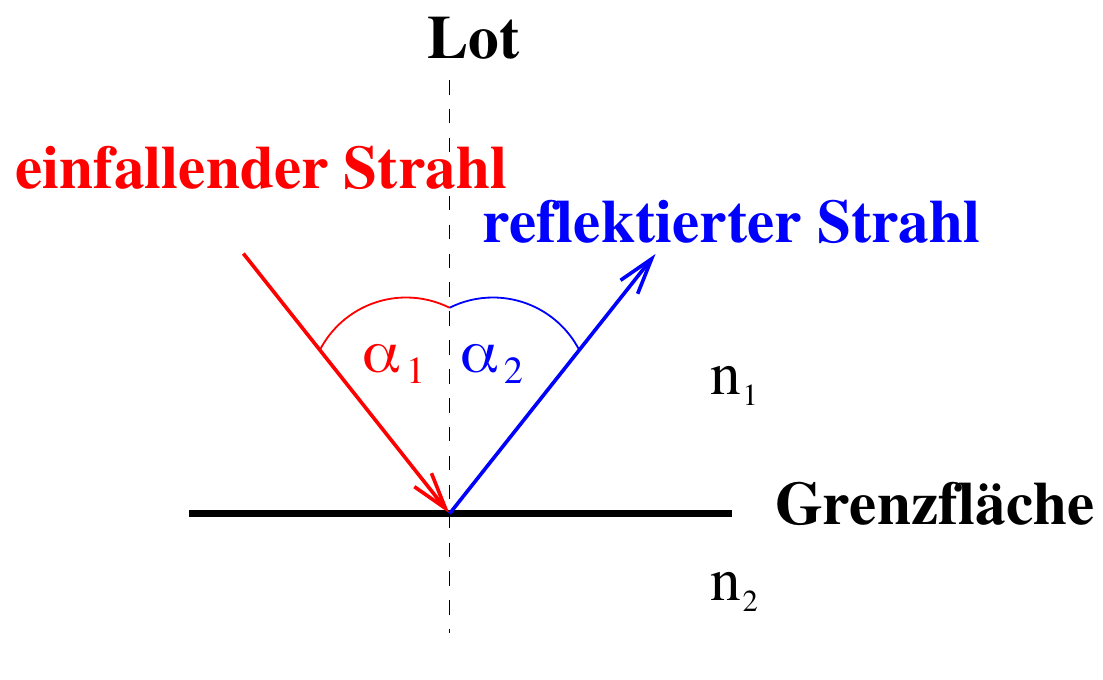
\includegraphics[scale = 0.3]{pictures/Reflexion.png}
    \caption{Reflexion eines Lichtstrahls \cite{AP01}.}
    \label{fig:reflexion}
\end{figure}

\subsubsection*{Brechung}
\label{sec:brechung}
Die Ausbreitungsgeschwindigkeit von Licht hängt von dem Medium ab, in dem es sich bewegt. Wechselt ein Lichtstrahl
nun an einer Grenzfläche das Medium, kommt es zur Brechung des Strahls, da sich die Ausbreitungsgeschwindigkeit
ändert. Dabei berechnet sich das Verhältnis der Geschwindigkeiten zu den Winkeln des Lichtstrahls wie
\begin{equation}
    \frac{v_1}{v_2}=\frac{\sin\alpha}{\sin\beta}=\frac{n_2}{n_1}.
    \label{eqn:brechung1}
\end{equation}
Dabei wurde der Brechungsindex $n$ eingeführt, welcher als Materialeigenschaft den Zusammenhang \ref{eqn:brechung1}
bestmöglich beschreibt. Die Brechung eines Lichtstrahls an einer Grenzfläche zwischen zwei Medien mit verschiedenen
Brechungsindizes ist in Abbildung \ref{fig:brechung} dargestellt.
\begin{figure}[H]
    \centering
    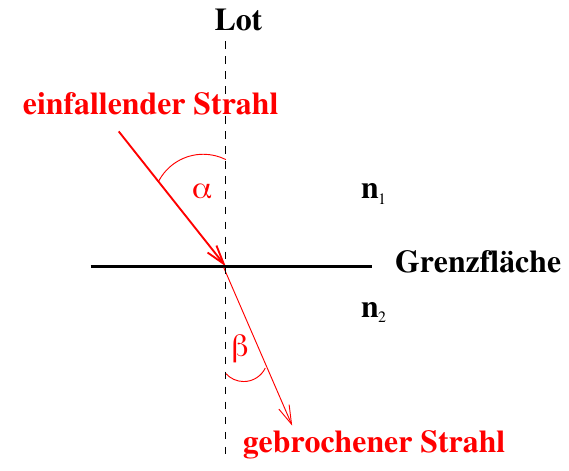
\includegraphics[scale = 0.5]{pictures/Brechung.png}
    \caption{Brechung eines Lichtstrahls \cite{AP01}.}
    \label{fig:brechung}
\end{figure}
\noindent
Der Brechungsindex von Luft liegt bei ca. $\num{1.000292}$ \cite{AP01} und ist daher für unsere Zwecke als $1$
anzusehen. Somit wird \eqref{eqn:brechung1} für $n_1\approx1$ zu
\begin{equation}
    \frac{\sin\alpha}{\sin\beta}=n_2.
    \label{eqn:brechung2}
\end{equation}
Die Ausbreitungsgeschwindigkeit von Licht in einem Medium hängt jedoch nicht nur von dem Brechungsindex des Mediums
ab, sondern auch von der Wellenlänge $\lambda$ des Lichtstrahls. Somit verändert sich auch das Brechungsverhalten.
Diese Abhängigkeit wird Dispersion genannt und wird erneut in Kapitel \ref{sec:prisma} aufgegriffen.

\subsubsection*{Reflexion und Transmission}
\label{sec:RefTrans}
Allgemein finden sowohl Reflexion, als auch Transmission und Brechung statt, wenn ein Lichtstrahl auf eine Grenzfläche zweier
Medien trifft. Ein gewisser Anteil der Intensität $R$ wird an der Grenzfläche reflektiert und der restliche
Teil der Intensität $T$ transmittiert durch die Grenzfläche und wird gebrochen. Da bei diesem Prozess die
Summe der Intensität erhalten bleibt gilt
\begin{equation}
    R+T=1.
\end{equation}
Wie nun die Intensität verteilt ist, hängt von den Materialien ab. In Abbildung \ref{fig:RefTrans}
sind die beiden Prozesse aus Abbildung \ref{fig:reflexion} und \ref{fig:brechung} zusammen dargestellt.
\begin{figure}[H]
    \centering
    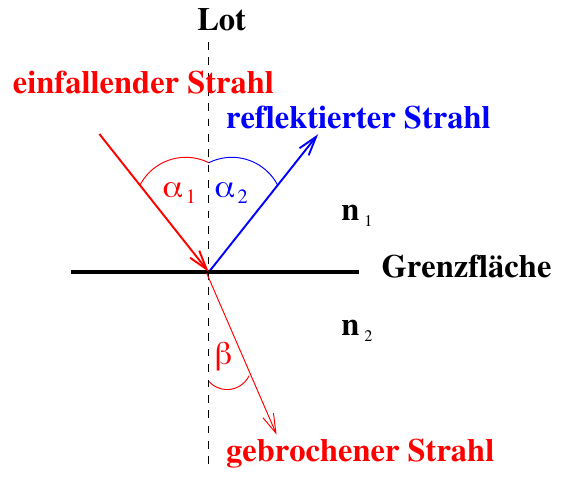
\includegraphics[scale = 0.5]{pictures/ReflexionTransmission.png}
    \caption{Reflexion und Transmission eines Lichtstrahls \cite{AP01}.}
    \label{fig:RefTrans}
\end{figure}

\subsection{Beugung}
\label{sec:beugung}
Um das Phänomen der Beugung zu erklären, reicht die einfache Strahlenoptik nicht aus. Hier muss auf die Wellenoptik
zurückgegriffen werden. Als Beugung oder auch Diffraktion wird das Ausbreiten einer Welle hinter einem
Hindernis bezeichnet. In diesem Raum hinter dem Hindernis kann sich ein geradliniger Strahl nicht ausbreiten, die Beugung ist
also ein Wellenphänomen. Um Aussagen über das Verhalten der Welle bei einer Beugung zu machen, wird das Huygensche
Prinzip verwendet. Dieses besagt, dass jeder Punkt der Wellenfront ein Ausgangspunkt für eine sich um den Punkt kreisförmig
ausbreitenden Welle ist. Diese sich ausbreitende Welle besitzt diesselbe Frequenz wie die, aus der sie hervorgegangen
ist. Primär- und Sekundärwelle haben eine feste Phasenbeziehung zueinander. Aus der Einhüllenden aller so
entstandenen Sekundärwellen bildet sich die neue Wellenfront. Bei einem Spalt der Breite $a$ wird auf einem Schirm
im Abstand $L$ das $k$-te Intensitätsmaximum der gebeugten Welle bei
\begin{equation}
  \label{eqn:spaltintmax}
  a \cdot \sin(\alpha) = k \cdot \lambda
\end{equation}
gemessen. Hierbei bezeichnet $\alpha$ den Winkel relativ zur orthogonal zum Schirm verlaufenden Ausbreitungsrichtung
und $\lambda$ die Wellenlänge der einlaufenden Welle.
Im Falle eines Gitters mit senkrecht einlaufenden Wellen wird das $k$-te Intensitätsmaximum auf dem Schirm bei
\begin{equation}
  \label{eqn:gitterintmax}
  d \cdot \sin(\alpha) = k \cdot \lambda
\end{equation}
gemessen, wobei hier $d$ die Gitterkonstante bezeichnet.

\subsection{Optische Elemente}
\label{sec:optischeelemente}

\subsubsection*{Planparallele Platten}
\label{sec:platten}
Bei einer planparallenen Platte handelt es sich um einen flachen, transparenten Quader. Tritt Licht in die Platte ein, wird
es gemäß \ref{sec:brechung} gebrochen. Zudem wird es auch beim Austritt gebrochen, sodass der Strahl seinen Winkel und
somit auch seine Richtung nicht verändert. Es entsteht lediglich ein Strahlenversatz, der durch
\begin{equation}
    s=d\frac{\sin(\alpha-\beta)}{\cos\beta}
    \label{eqn:strahlenversatz}
\end{equation}
berechnet werden kann. In Abbildung \ref{fig:platten} ist der Strahlenverlauf noch einmal schematisch dargestellt.
\begin{figure}[H]
    \centering
    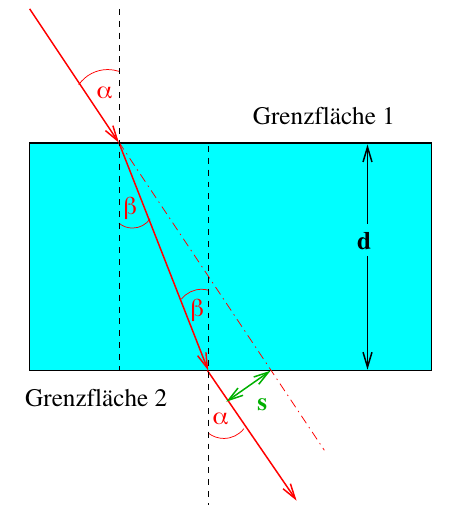
\includegraphics[scale = 0.5]{pictures/Platte.png}
    \caption{Brechung eines Lichtstrahls in einer planparallelen Platte \cite{AP01}.}
    \label{fig:platten}
\end{figure}

\subsubsection*{Prisma}
\label{sec:prisma}
Ein Prisma ist ein optisches Element, welches die geometrische Form eines Prismas mit einem Dreieck als Grundfläche
besitzt. Somit besitzt das Prisma nicht parallele Flächen, welche im sogenannten
brechenden Winkel $\gamma$ zueinander stehen.
\\\noindent
Trifft ein Lichtstrahl auf eine der Flächen, wird ein Teil nach Kapitel
\ref{sec:brechung} gebrochen. Dies geschieht sowohl beim Eintritt als auch beim Austritt aus dem Prisma. Dabei wird
der Lichtstrahl um den Winkel $\delta$ abgelenkt. Dieser lässt sich durch
\begin{equation}
    \delta=(\alpha_1+\alpha_2)-(\beta_1-\beta_2)
    \label{eqn:ablenkwinkel}
\end{equation}
berechnen. In Abbildung \ref{fig:prisma2} ist dies nocheinmal schematisch verdeutlicht.
\begin{figure}[H]
    \centering
    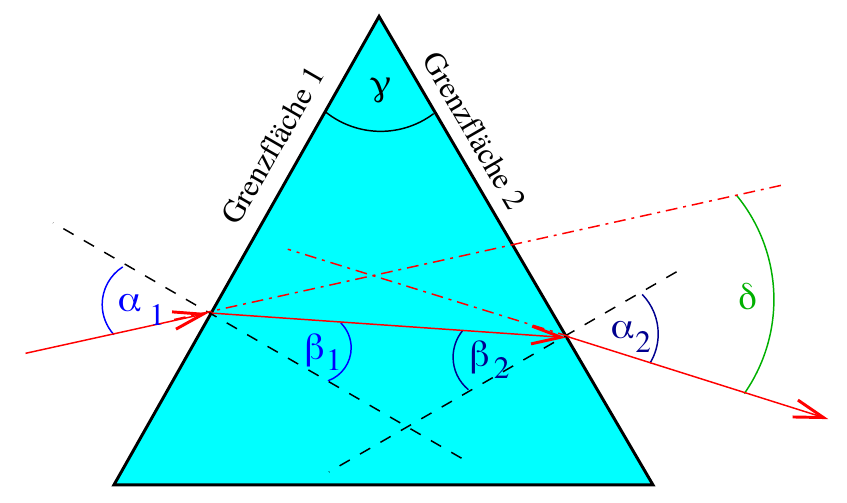
\includegraphics[scale = 0.4]{pictures/Prisma.png}
    \caption{Brechung eines Lichtstrahls im Prisma \cite{AP01}.}
    \label{fig:prisma2}
\end{figure}
\noindent
Wie bereits in Kapitel \ref{sec:brechung} beschrieben, hat die Wellenlänge einen Einfluss auf das Brechungsverhalten.
Gerade bei einem Prisma wird dies besonders deutlich, da durch die geometrische Form die Ablenkwinkel verschiedener
Wellenlängen so unterschiedlich sind, dass polychromatisches Licht beim Einfall in seine Spektralfarben zerlegt wird.
